\documentclass[12pt,letterpaper]{article}

\usepackage[authoryear]{natbib}
\usepackage{times} 
\usepackage{amsmath,amsfonts}
\usepackage{graphicx}
\usepackage{setspace}
\usepackage{indentfirst}
\usepackage{color}
\usepackage{lscape}
\usepackage[paper=letterpaper]{geometry}

% revise margins
\setlength{\headheight}{0.0in}
\setlength{\headsep}{0.0in}
\setlength{\topmargin}{0.0in}
\setlength{\textheight}{8.9in}
\setlength{\footskip}{0.4in}
\setlength{\oddsidemargin}{0.1in}
\setlength{\evensidemargin}{0.1in}
\setlength{\textwidth}{6.3in}

\setlength{\rightskip}{0pt plus 1fil} % makes ragged right

% bibliography format
\usepackage[authoryear]{natbib}
\bibpunct{(}{)}{;}{a}{}{,}

 
% hanging environment for Figure legends
\newenvironment{hanging}
{\begin{list}{}
        {\setlength{\labelwidth}{0in}
         \setlength{\leftmargin}{1em}
         \setlength{\itemindent}{-1em}
        }
}
{\end{list}}

\begin{document}
\setstretch{2.0}

\vspace*{8mm}
\begin{center}

\textbf{\Large Genotype probabilities at intermediate generations\\[18pt]
in the construction of recombinant inbred lines}
 
 
\bigskip \bigskip \bigskip \bigskip 
 
{\large Karl W. Broman$^1$

\bigskip \bigskip

Department of Biostatistics and Medical Informatics, \\
University of Wisconsin--Madison, Madison, Wisconsin 53706 }
\end{center}


\vfill

\hfill 
{\footnotesize 14 November 2011}

\newpage

\noindent \textbf{Running head:} 
Pre-CC genotype probabilities


\bigskip \bigskip \bigskip

\noindent \textbf{Key words:} recombinant inbred lines, Collaborative
Cross, Markov chains, recursion, map expansion, fixation




\bigskip \bigskip \bigskip

\noindent \textbf{$^1$Corresponding author:}

\begin{tabular}{lll}
 \\
 \hspace{1cm} & \multicolumn{2}{l}{Karl W Broman} \\
 & \multicolumn{2}{l}{Department of Biostatistics and Medical Informatics} \\
 & \multicolumn{2}{l}{University of Wisconsin--Madison} \\
 & \multicolumn{2}{l}{1300 University Ave, Rm 4710 MSC} \\
 & \multicolumn{2}{l}{Madison, WI 53706} \\
 \\
 & Phone: & 608--262--4633 \\
 & Fax: & 608--265--7916 \\
 & Email: & \verb|kbroman@biostat.wisc.edu|
\end{tabular}


\clearpage
\centerline{ABSTRACT} 
  
The mouse Collaborative Cross (CC) is a panel of eight-way recombinant
inbred lines: eight diverse parental strains are intermated, followed
by repeated sibling mating, many times in parallel, to create a new
set of inbred lines whose genomes are random mosaics of the genomes of
the original eight strains.  Many generations are required to reach
inbreeding, and so a number of investigators have sought to make use
of phenotype and genotype data on mice from intermediate generations
during the formation of the CC lines (so-called pre-CC mice).  The
development of a hidden Markov model for genotype reconstruction in
such pre-CC mice, on the basis of incompletely informative genetic
markers (such as single nucleotide polymorphisms), formally requires
the two-locus genotype probabilities at an arbitrary generation along
the path to inbreeding.  In this paper, I describe my efforts to
calculate such probabilities.  While closed-form solutions for the
two-locus genotype probabilities could not be derived, I provide a prescription for
calculating such probabilities numerically.  In addition, I present a
number of useful quantities, including single-locus genotype
probabilities, two-locus haplotype probabilities, and the fixation
probability and map expansion at each generation along the course to
inbreeding.



\clearpage
\centerline{INTRODUCTION}

The mouse Collaborative Cross (CC) is a panel of eight-way recombinant
inbred lines (RIL): eight diverse parental strains are intermated,
followed by repeated sibling mating, many times in parallel (see Figure~1D), to create
a new set of inbred lines whose genomes are random mosaics of the
genomes of the original eight strains \citep{CTC2004,CC-CROSS-CC1}. There are
similar efforts for Drosophila \citep{Macdonald2007} and Arabidopsis
\citep{Kover2009}; the panels will serve as important reference
populations for the system genetic analysis of complex traits.

Many generations are required for inbreeding of such RIL, and so
a number of investigators have sought to make use of phenotype
and genotype data on mice from intermediate generations during the
formation of the CC lines: the pre-CC mice \citep[e.g.,
see][]{Aylor2011}.  The mapping of quantitative trait loci (QTL)
with data on pre-CC mice, whether by interval
mapping \citep{Lander1989} or Haley-Knott regression
\citep{Haley1992}, requires the calculation of conditional
genotype probabilities given incompletely informative marker data
(e.g., at single nucleotide polymorphisms).  Such probabilities are generally derived using a
hidden Markov model (HMM).  The construction of an HMM for pre-CC mice
formally requires the calculation of two-locus diplotype 
probabilities
at arbitrary generations along the course to inbreeding.
Thus, I sought to calculate single-locus genotype probabilities and
two-locus diplotype probabilities at generation $\text{G}_2:\text{F}_k$ (see Fig.~\ref{fig:rifig}D),
with the latter being a function of the recombination fraction between
the two loci.  

Previous work on genotype probabilities in RIL has focused largely on
the final lines \citep{Haldane1931, Broman2005, Teuscher2007}, though
\citet{Haldane1931} did calculate a portion of the probabilities for
intermediate generations in two-way RIL by selfing.  More recently, 
\citet{Johannes2011} fully derived the two-locus genotype
probabilities for two-way RIL by selfing and described numerical
calculations for the autosome in two-way RIL by sibling mating.

Here I extend these results to the case of four- and eight-way RIL by selfing
and sibling mating, including consideration of the X chromosome.  
The basic problem is to calculate the $k$-step probabilities of a
Markov chain with many states.  
While I was not able to obtain closed-form solutions for the
two-locus diplotype probabilities at $\text{F}_k$ in
RIL by sibling mating, I do
provide recipes for calculating the probabilities numerically.  
And I was able to obtain closed-form solutions for single-locus
genotype probabilities and two-locus haplotype probabilities.
Further, I derived the fixation probability and map expansion 
at $\text{F}_k$.  These latter results have important applications: the
single-locus genotype probabilities could be useful in efforts to
identify regions under selection, through the comparison of
observed to expected genotype frequencies; the fixation probability can be 
interpreted as the expected proportion of the genome that is fixed;
and the map expansion results indicate the accumulation of
recombination events over generations.


\clearpage
\centerline{METHODS}

The generation of two-way RIL by
selfing, and of two-, four- and eight-way RIL by sibling mating, is
shown in Figure~\ref{fig:rifig}.  The notation for generation
numbers for RIL can be confusing.  The
numbering indicated in Figure~\ref{fig:rifig} will be used throughout, with $\text{F}_1$ being
the first generation in which all parental alleles are present in a
single individual.  In the following, I will abbreviate
$\text{G}_1:\text{F}_k$ in four-way RIL and $\text{G}_2:\text{F}_k$ in
eight-way RIL as simply $\text{F}_k$.  In particular, $\text{G}_1$ in
four-way RIL and $\text{G}_2$ in eight-way RIL will be called
$\text{F}_0$.  

Consider a particular crossing strategy, and let $X_k$ denote the
parental type at generation $\text{F}_k$.  For RIL by selfing, this is
the diplotype of the individual; for RIL by sibling mating, this is
the pair of diplotypes for the two siblings.  For example, in
considering two loci in four-way RIL by sibling mating, one possible
state is the starting state at $\text{F}_0$, $AA|BB \times CC|DD$.
(In this notation, the pairs of letters
on each side of the vertical bar denote the two haplotypes for an
individual; the first and second letters in each haplotype correspond
to the alleles at the first and second loci, respectively.)  The
sequence $X_0, X_1, X_2, \dots$, form a Markov chain.  That is,
$X_{k+1}$ is conditionally independent of $X_0, X_1, \dots, X_{k-1}$,
given $X_k$.

Let $P$ denote the transition matrix of the Markov chain, defined by $P_{ij} =
\Pr(X_{k+1} = j | X_k = i)$.  Our goal is to calculate the $k$-step
probabilities, $\pi_k = \pi_0
P^k$, where $\pi_0$ is the starting distribution (at
$\text{F}_0$), which contains 1 at the fixed starting
state and 0 for all other states.

First note that, for RIL by selfing, it is sufficient to consider
two-way RIL, and for RIL by sibling mating, it is sufficient to
consider four-way RIL.  This is due to the bottleneck with two
chromosomes in RIL by selfing at generation $\text{F}_1$ and with four
chromosomes in RIL by sibling mating at generation $\text{F}_0$.  The
results may be extended from two-way RIL by selfing to four-way RIL by
selfing, or from four-way RIL by sibling mating to eight-way RIL by
sibling mating, by considering an additional generation of
recombination.  One may
obtain the results for two-way RIL by sibling mating from the results
for four-way RIL by sibling mating
by collapsing states: let $A \equiv B$ and $C \equiv D$.

The major technique for deriving the $k$-step probabilities, $\pi_k$,
is to derive the eigen decomposition of the transition matrix: $P = V
\Lambda V^{-1}$, where $\Lambda$ is the diagonal matrix of eigenvalues and $V$ is
a matrix whose columns are the corresponding eigenvectors.  Then $P^k
= V \Lambda^k V^{-1}$, and $\Lambda^k$ is obtained from $\Lambda$ by taking the
$k$th powers of the eigenvalues.

Such an eigen decomposition is straightforward in theory but is
unwieldy in practice, due to the extremely large number of possible
states.  And so the second major technique is to take account of
various symmetries to collapse the states into a smaller number.  For
two-way RIL by selfing with two loci, the simplest formulation would
give $2^4 = 16$ possible states (two possible alleles at each locus on
each of the two chromosomes).  But considering that the order of the two
haplotypes is immaterial, these may be reduced to 10 possible
diplotypes.  As shown in \citet{Haldane1931}, these may be further
reduced to just five states, by taking account of two additional
symmetries: the order of the two loci may be ignored, and the symbols
$A$ and $B$ may be switched.  

Let us formalize this idea.  (For a more rigorous approach, see
\citet{Burke1958}.)  Let the possible states of the chain be $S =
\{s_1, \dots, s_n\}$.  Partition $S$ into $m$ subsets of equivalent
states, $S_i \subset S$, so that, for any pair $i$ and $j$,
$\Pr(X_{k+1} \in S_j | X_k = s) = q_{ij}$ for all $s \in S_i$.
The $q_{ij}$ form an $m \times m$ transition matrix, $Q$, for the
collapsed states.  Let $Z$ denote the $n \times m$ incidence matrix
defined by $z_{ij} = 1$ if $s_i \in S_j$ and 0 otherwise.  Then 
\begin{eqnarray}
PZ & = & ZQ
\end{eqnarray}
and so $P^kZ = ZQ^k$.  As a result, $\pi_k Z = \pi_0 P^k Z =
\pi_0 Z Q^k$.  Thus, one may work with the $m \times m$ transition
matrix $Q$ in place of the $n \times n$ transition matrix $P$.  

For this collapse of states to be useful, 
the multiple states within each
equivalence class, $S_i$, need to have equal probabilities at each
generation, so that the probabilities of the individual
states may be derived from the probabilities of the collapsed states.  This will
depend on the starting distribution.  For example, consider one locus
in two-way RIL by sibling mating.  If the starting state is $AA \times
BB$, then at any future generation, the chance of being in state $AA
\times AB$ is the same as that of state $AB \times BB$.  However, if
the starting state is $AA \times AB$, then there will be a lack of symmetry
between $A$ and $B$. (For the asymmetric case of two-way RIL initiated
from a backcross, see \citet{Johannes2011}.)

\citet{Kimura1963} described a further technique that has been
critical in this work.  In many instances, we do not need the full
distribution $\pi_k$, but only various linear combinations, say
$\pi_k z = \pi_0 P^k z$, where $z$ is an $n \times 1$ vector.
\citet{Kimura1963} demonstrated how to expand $z$ to an $n \times m$
matrix $Z$ in such a way that there exists a matrix $Q$ satisfying
equation (1).  Then we again have $\pi_k Z = \pi_0 P^k Z = \pi_0 Z
Q^k$ and may work with the $m \times m$ matrix $Q$ in place of the $n
\times n$ matrix $P$.  Here, the matrix $Q$ is not a transition matrix
but simply defines a recursion.  The first element of $\pi_k Z$ is the
target quantity, $\pi_k z$.

Consider, for example, the probability of a random two-locus haplotype
drawn from generation $\text{F}_k$ in the formation of RIL by sibling mating.
Let $C_k(AA)$ denote that chance that $AA$ is drawn.  This could
either be an intact haplotype, transmitted without recombination from
generation $\text{F}_{k-1}$, or it is the result of recombination
between the two haplotypes in a random $\text{F}_{k-1}$ individual.
Consider drawing a single random allele at the first locus from
generation $k$, and then taking the allele at the second locus but on
the opposite chromosome in that individual.  Let $S_k(AA)$ denote the
probability that these two alleles are both $A$.  Then $C_k(AA) =
(1-r)C_{k-1}(AA) + r S_{k-1}(AA)$, where $r$ is the recombination
fraction between the two loci.  Further, $S_k(AA) = T_{k-1}(AA)$,
where $T_k(AA)$ is the chance that, if one draws a random allele at the
first locus from generation $\text{F}_k$ and then a random allele from
the opposite individual at the second locus, both alleles are $A$.  We
may further write $T_k(AA)$ as a function of $C_{k-1}$, $S_{k-1}$,
and $T_{k-1}$, forming the recursion matrix, $Q$, which is shown in the
supplementary information (Table~S1).  Moreover, this same recursion
applies for all of the other haplotypes; one just needs to use different
starting distributions, $\pi_0 Z$.  For the three distinct cases for
four-way RIL by sibling mating, these are shown in Table~S2.

A particularly useful aspect of Kimura's technique is that 
the recursion matrix can be constructed by probabilistic arguments, without the
need to form the full transition matrix, $P$, or even the $n \times m$
matrix $Z$.  For two autosomal loci in four-way RIL by sibling mating,
there are $4^8 = 65,536$ diplotype pairs without accounting for
any symmetries.  This may be reduced to 9,316 after accounting for the
obvious symmetries (exchange the two haplotypes in each individual and
exchange the two individuals), and then to 700 diplotype states after
accounting for the less obvious symmetries (exchange the two loci,
exchange alleles $A$ and $B$, exchange alleles $C$ and $D$, and
exchange both $A$ for $C$ and $B$ for $D$).  By the technique of
\citet{Kimura1963}, 
one may work with a $3 \times 3$ matrix in place of the $700
\times 700$ transition matrix, if only haplotype probabilities are
desired.  

Throughout this work, Maxima \citep{Maxima} was used 
for symbolic algebra, and R \citep{R} and Perl \citep{Perl} were used for
additional verifications of the results.


\clearpage
\centerline{RESULTS}

\textbf{Two-way RIL by selfing:} As noted in the previous section, it
is sufficient to consider two-way RIL by selfing, due to the
bottleneck with two chromosomes at $\text{F}_1$.  Let us jump
directly to two-locus diplotype probabilities, as the results are
fairly simply obtained.  As noted in \citet{Haldane1931} and in the
previous section, if one takes account of the various symmetries, one
may collapse the two-locus diplotype states to a Markov chain with
five states.  The transition matrix of this chain is shown in the
supplementary material, in Table~S3, with $r$ denoting the
recombination fraction between the two loci.

I obtained the eigen decomposition of this transition matrix (not shown), and noting
that the starting state (at generation $\text{F}_1$) is $AA|BB$, 
derived the two-locus diplotype probabilities at generation $\text{F}_k$
(that is, after $k-1$ steps), $\pi_{k-1} = \pi_0 P^{k-1} = \pi_0 V
\Lambda^{k-1} V^{-1}$, presented in Table~1.  For each group of
states, a single prototype and the number
of states in that group is provided. For example, in the third row, with prototype
$AA|AB$, the cited probability is for that prototype as well as each of the
other three states in that group: $AA|BA$, $BB|AB$ and $BB|BA$.  

\citet{Haldane1931} also derived these results for intermediate
generations in two-way RIL by selfing.  They displayed just the two
cases $AA|AA$ and $AB|AB$ \citep[][equation 1.4]{Haldane1931}, but the
results match those in Table~1, though note that their results are a
factor of two larger, as they concern the combined states.  Also note
that \citet{Haldane1931} allowed a sex difference in the recombination
fraction, whereas I assume no sex difference in recombination.  




\textbf{Four-way RIL by sibling mating, one locus:} \emph{Autosome:}
For a single autosomal locus in four-way RIL by sibling mating, there
are 55 genotype pairs, after accounting for the obvious symmetries.
These may be reduced to 13 states, after accounting for the less
obvious symmetries.  The transition matrix for this reduced Markov
chain is shown in Table~S4.  The starting state at generation
$\text{F}_0$ is $AB \times CD$.  I calculated the eigen decomposition
of the transition matrix, and from that $\pi_k = \pi_0 P^k = \pi_0 V
\Lambda^k V^{-1}$.  The results are shown in Table~S5, which also
indicates the number of genotype pairs corresponding to each of the 13
states.  (The sum of the second column in Table~S5 is 55.)

The probabilities of single-locus genotype pairs at generation $\text{F}_{k}$,
shown in Table~S5, are complex and not of particular interest in
themselves (hence their inclusion in the supplementary
material). However, the
single-locus probabilities for a random $\text{F}_k$ individual follow
immediately from these results; they 
are shown in Table~2.  These are of considerably greater interest, as
they constitute the ``initiation'' probabilities for an HMM.
The single-locus genotype probabilities for the first several
generations are plotted in Figure~S1A.





\emph{X chromosome:} 
In considering the X chromosome, it is important to consider the order
of the initial crosses.  In four-way RIL by sibling mating, I assume
that a female $A$ was crossed to a male $B$, and a female $C$ was
crossed to a male $D$, and then a female from the $A \times B$
$\text{F}_1$ was crossed to a male from the  $C \times D$ $\text{F}_1$
(see Figure~S2B).  In the F$_1$, there are three X chromosomes: $A$,
$B$ and $C$; the $D$ allele is lost.  

After accounting for the obvious symmetries, there are 18 possible
single-locus genotype pairs. 
These may be reduced to 10 states, after
accounting for the less obvious symmetries.  The transition matrix for
this reduced Markov chain is shown in Table~S6.  The starting state at
generation $\text{F}_0$ is $AB \times C$.  Through the eigen
decomposition of the transition matrix, the results in
Table~S7 are obtained.  

The marginal probabilities for the female and male are displayed in
Table~2, and are plotted in Figure~S1B and S1C.  The oscillations in
the male X chromosome probabilities are interesting, but not
particularly surprising.



\emph{Fixation probabilities:} The detailed single-locus results in
Tables~S5 (for autosomes) and S7 (for the X chromosome) immediately
provide the fixation probability in four-way RIL by sibling mating.
For an arbitrary autosomal locus, the chance that a four-way RIL has
been fixed at or before generation $\text{F}_k$ is $4 \cdot
\Pr(AA \times AA)$. For an arbitrary X chromosome locus, the chance of
fixation by generation $\text{F}_k$ is $2 \cdot \Pr(AA \times A) +
\Pr(CC \times C)$.  These are shown in Table~3 and are further plotted
in Figure~\ref{fig:fixation}A.  Note that the
probability that an arbitrary locus in four-way RIL has become fixed
at exactly generation $\text{F}_k$ may be derived as the difference between the results
for $k$ and $k-1$.  These are shown in Figure~\ref{fig:fixation}B.
Note that the fixation probabilities for eight-way RIL are identical
to those for four-way RIL.

The fixation probabilities for two-way RIL by sibling mating are also
simply derived: collapse alleles $A \equiv B$ and $C \equiv
D$.  Thus, for an autosomal locus, one adds up the rows in Table~S5 
that contain only $A$ or $B$.

The fixation probability for an X chromosome locus is slightly larger
than that for an autosomal locus, and that for two-way RIL is slightly
larger than that for four-way RIL.  The fixation probability for
two-way RIL by sibling mating at generation $k$ is quite similar to that of 
four-way RIL at generation $k+1$.  Fixation in RIL by
selfing occurs much more rapidly.  

For a large genome, the fixation probabilities for an arbitrary
autosomal locus, displayed in Figure~\ref{fig:fixation}A, may be
interpreted as the approximate proportion of the autosomal genome that
will be fixed at generation $\text{F}_k$.  Nevertheless, as shown in
\citet{Broman2005} via computer simulation, there will be considerable
variation across lines.



\textbf{Four-way RIL by sibling mating, two-locus haplotypes:}
\emph{Autosome:} The technique of \citet{Kimura1963}, described above,
may be used to derive probabilities of random two-locus haplotypes
drawn from generation $\text{F}_k$ in the formation of four-way RIL by
sibling mating.  There are three distinct cases to consider ($AA$,
$AB$, and $AC$), which share a common recursion matrix (shown in
Table~S1) but require consideration of different starting states.  For
each case, the starting probabilities, $\pi_0 Z$, form a $1 \times 4$
row vector with a single non-zero entry (see Table~S2).

I obtained the eigen decomposition of the recursion matrix, $Q$, that
is shown in
Table~S1, and through the equation $\pi_k Z = \pi_0 Z Q^k = \pi_0 Z V
\Lambda^k V^{-1}$, obtained the two-locus haplotype probabilities in Table~4.  
The equations for autosomal haplotypes in Table~4 are valid only for
$r < 1/2$, but the results for $r=1/2$ are obvious by symmetry:
$\Pr(AA)=1/4$ at $\text{F}_0$, $\Pr(AA) = \Pr(AB) = 1/8$ at
$\text{F}_1$, and $\Pr(AA) = \Pr(AB) = \Pr(AC) = 1/16$ at $\text{F}_k$
for $k \ge 2$.  

The autosomal haplotype probabilities as a function of the
recombination fraction, $r$, are displayed in the left panels in
Figure~S3. 

\emph{X chromosome:} To calculate the probability of a random
two-locus X chromosome haplotype drawn from the female
at $\text{F}_k$ in four-way RIL by sibling mating, and of the single X
chromosome haplotype in the corresponding male, there
are four cases to consider ($AA$, $AB$, $AC$, and $CC$).  
Application of the technique of \citet{Kimura1963} for the X chromosome
requires consideration of a set of four states, with the recursion
matrix shown in Table~S8.  Each of the four cases uses the same
recursion matrix but different starting probabilities (shown in
Table~S9).  Calculation of the probabilities of a random haplotype drawn
from the female and of the single haplotype in the male use the same
set of equations, but for a random female haplotype one takes the first
element of $\pi_k Z$, while for the male haplotype one takes the third element.
Again, following the eigen decomposition of the matrix in Table~S8, 
the haplotype probabilities in Table~4 were obtained.


The female and male X chromosome haplotype probabilities, as a function
of the recombination fraction, $r$, are displayed in the middle
and right panels, respectively, in Figure~S3.  The probabilities of
haplotypes $AA$ and $CC$ in females, and all of the haplotype
probabilities in males, show pronounced oscillations across generations.
For example, the $CC$
haplotype is common in males for even $k$ and common in females for
odd $k$, and vice versa for haplotype $AA$.


\emph{Map expansion:} The multiple generations of recombination in the
formation of RIL lead to genetic map expansion.  
The map expansion as a function of generation is
easily obtained from the haplotype probabilities.  Let $R$ denote the
probability of a recombinant haplotype.  (For the autosome, take $1 - 4
\cdot \Pr(AA)$.)  The map expansion relative to a single meiosis is
$\left. \frac{dR}{dr} \right|_{r=0}$ \citep[see][]{Teuscher2007}.
For the X chromosome, I calculated the map expansion separately in
females and males and then obtained a combined map expansion by
averaging the two values, giving the female value weight 2/3.

The map expansion for the two-way RIL by selfing case may be obtained
from the values in Table~1.  To obtain the map expansion for two-way RIL by
sibling mating, equate alleles $A \equiv B$ and $C \equiv D$;
the recombinant haplotypes correspond to the $AC$ case in Table~4.
To obtain the map expansion for eight-way RIL by sibling mating, 
note that the chance of each non-recombinant haplotypes would be
$(1-r)/2$ times the probability for haplotype $AA$ shown in Table~4.
A similar calculation applies for four-way and eight-way RIL by
selfing.  

The map expansions for two-, four-, eight-way, and $2^n$-way RIL by
selfing and for the autosome by sibling mating are shown in Table~5
and are further illustrated in Figure~\ref{fig:mapexpansion}.  The
results for the X chromosome in RIL by sibling mating are simply 2/3
those for the autosome, and so are not shown.  (I have verified, via
Maxima, that this is true for $2^n$-way RIL up to $n=98$.  A general
proof continues to elude me.)

\citet{Teuscher2005} had also sought to calculate the map expansion by
generation for two-way RIL by sibling mating.  My results match those
of \citet{Teuscher2005}, were more easily obtained, and provide
a closed-form solution.



\textbf{Four-way RIL by sibling mating, two-locus diplotypes:}
\emph{Autosome:} I now turn to the calculation of the distribution of
the two-locus diplotype on an autosome, for a random individual drawn
from generation $\text{F}_k$ in the formation of four-way RIL by
sibling mating.  There are 18 cases falling into
three groups: diplotypes of the form $AA|AA$, with both loci being
homozygous; $AA|AB$, with one locus being homozygous; and $AA|BB$,
with both loci being heterozygous.  

Let us start with the $AA|AA$ case.  Following the approach of
\citet{Kimura1963}, I obtained a $13 \times 13$ recursion matrix, $Q$,
whose transpose is shown in Table~S10.  Because of the size and
sparsity of the matrix, only the non-zero elements are indicated.  The
starting states for the three related diplotypes are shown in
Table~S11.  (For each diplotype pattern, the starting distribution
$\pi_0 Z$ has a single non-zero entry.)

The next step is to derive the eigen decomposition of
$Q$.  However, while 7 of the 13 eigenvalues can be obtained, the other
6 eigenvalues are the roots of a sixth degree polynomial (whose
coefficients are polynomials of $r$ of degree up to 5).  This prevented
the calculation of the diplotype probabilities at
$\text{F}_k$.  

Nevertheless, the reduction of states represented in Tables~S10 and
S11 is considerable, and is useful for the numeric calculation of
these probabilities.  Direct calculation would require
consideration of the full transition matrix for pairs of diplotypes,
which even after accounting for all possible symmetries, is a $700
\times 700$ matrix.  

Turning to the $AA|AB$ case, with one locus being homozygous and the
other heterozygous, the recursion matrix is $17
\times 17$; the non-zero elements of its transpose
are shown in Table~S12.
The starting states for the four related
diplotype patterns are shown in Table~S13.

Finally, for the $AA|BB$ case, with both loci being heterozygous, the
recursion matrix is $14 \times 14$; its transpose is shown in 
Table~S14.  The starting states for the 11 related diplotype patterns
are shown in Table~S15.  



\emph{X chromosome:}  It should not be surprising that closed-form
solutions for the two-locus diplotype
probabilities for the female on the X chromosome at generation
$\text{F}_k$ in the formation of four-way RIL by sibling mating could
not be derived.
(But
note that the probabilities for two-locus haplotype for the
male X chromosome could be calculated; see Table~5.)

Nevertheless, the recursion matrices and starting states,
derived by the approach of \citet{Kimura1963}, may be useful for
numerical computations.  After consideration of
the various symmetries, there are 17 two-locus diplotype patterns falling
into the same three groups as for the
autosome.  

For the $AA|AA$ case, the recursion matrix is $13 \times 13$; its 
transpose is shown in Table~S16.  The starting states for the
four related diplotype patterns are shown in Table~S17.  
Six of the 13 eigenvalues may be derived; the other seven are roots of a pair
of polynomials, one of degree 3 and the other of degree 4.  

For the $AA|AB$ case, the recursion matrix is $18 \times 18$; its
transpose is shown in Table~S18.  The starting states for
the five related diplotype patterns are shown in Table~S19.  For the
$AA|BB$ case, the recursion matrix is $12 \times 12$; its 
transpose is shown in Table~S20.  The starting states for the
eight related diplotype patterns are shown in Table~S21.



\textbf{Eight-way RIL:} The calculation of genotype or diplotype
probabilities for eight-way RIL from those for four-way RIL is
straightforward, but also tedious and potentially confusing.  For clarity,
lower case letters are used for the alleles in eight-way RIL, while
upper case letters denote the alleles in four-way RIL.

First, consider the genotype at an autosomal locus for a random
individual drawn from generation $\text{F}_k$ in the construction of
eight-way RIL by sibling mating.  Due to the bottleneck at generation
$\text{G}_2$, the genotypes $ab$, $cd$, $ef$, and $gh$ are not
possible.  (At any one locus, only one allele from each of these pairs
will be transmitted from $\text{G}_1$ to $\text{G}_2$.)  The
probability of genotype $aa$ is the chance that the $\text{G}_2$
individual receives the allele $a$ (which is 1/2) times the probability for the
genotype $AA$ in the construction of four-way RIL by sibling mating.
The probabilities of genotypes $ac$ and $ae$ are 1/4 the probabilities
of genotypes $AB$ and $AC$, respectively, in the construction of
four-way RIL by sibling mating.

Two-locus haplotype probabilities are obtained in a similar way,
noting that the haplotype in the position of the $A$ haplotype at
$\text{G}_2$ in the construction of four-way RIL is $aa$ or $bb$ with
probability $(1-r)/2$ each, and is $ab$ or $ba$ with probability $r/2$
each.  Thus, for example, the chance of obtaining $ab$ as a two-locus autosomal
haplotype, drawn at random from generation $\text{F}_k$ in the
construction of eight-way RIL by sibling mating, is $r/2$ times the
probability of drawing $AA$ from generation $\text{F}_k$ in the
construction of four-way RIL by sibling mating.  The chance of drawing
the haplotype $cg$ is $1/4$ times the probability of drawing $BD$ from the
corresponding generation in the construction of four-way RIL.

Table~S22 contains a complete prescription for the
calculation of two-locus autosomal diplotype probabilities for
intermediate generations in the construction of eight-way RIL, on the
basis of the corresponding probabilities for four-way RIL.  The first
column contains the possible diplotype patterns.  The second column
contains the numbers of diplotype states corresponding to each
pattern.  To calculate the probability of the pattern in the first
column, for an eight-way cross, take the corresponding probability
for the pattern in the third column, for a four-way cross, multiplied
by the value in the fourth column.

Table~S23 contains a similar prescription for calculating
probabilities of the two-locus X chromosome diplotype in the female at
intermediate generations in the construction of eight-way RIL.  A key
feature to note is that, at a single X chromosome locus at generation
$\text{G}_2$, the female is either $ac$ or $bc$, while the male is
hemizygous $e$ or $f$ (see Figure~S2C).





\clearpage
\centerline{DISCUSSION}


I sought to calculate the two-locus diplotype probabilities for a
random individual drawn from generation $\text{G}_2:\text{F}_k$ in the
formation of eight-way RIL by sibling mating, as these could form the
basis for an HMM for reconstructing the 
genotype probabilities in pre-CC individuals given incompletely
informative marker data.  While I was not able to obtain closed-form
solutions for these probabilities, the results in Tables~S10--S21
provide a recipe for numerical calculations.  


A more careful reading of \citet{Haldane1931} would have indicated
that closed-form solutions for these probabilities would not be
possible.  As they state \citep[p. 367]{Haldane1931}, regarding the
calculation of related probabilities for two-way RIL by sibling
mating, ``These equations can, in part at least, be reduced to
quartics, but at least one quartic is irreducible.  Hence only
numerical calculation is practicable.''

Moreover, \citet{Liu2010} described a general HMM for the treatment of complex
pedigrees with inbreeding, appropriate for pre-CC individuals, that
does not require the explicit derivation of these two-locus
probabilities.  Further, with the high-density genotype data
available on the pre-CC mice \citep{Aylor2011}, a relatively simple
HMM, such as that in HAPPY \citep{Mott2000}, which does not take
formal account of the varying recombination patterns as a function of
cross direction or generation, is likely sufficient for genotype
reconstruction.

Nevertheless, an HMM making use of these calculations, as well as
functions for simulating partially inbred lines, will be implemented
in a future version of R/qtl \citep{Broman2003}.  With this
implementation, we will be able to assess the relative advantages of such
a specially-tailored HMM over both the more general approach of
\citet{Liu2010} and the simpler approach of \citet{Mott2000}.

In practice, the genetic analysis of RIL generally proceeds prior to
full inbreeding, with calculations based on the haplotype
frequencies at fixation, and with remaining heterozygous genotypes
often omitted and treated as missing.  The calculations herein might
be used to deal with residual heterozygosity, but it is unlikely that
it will give much improvement in the analysis.  After only a few
generations, the haplotype probabilities are quite close to the values
at fixation.  Moreover, the consideration of heterozygotes can lead to
problems in the QTL analysis if the frequency of heterozygotes are
low, though this can be alleviated by an assumption of additive allele
effects at a QTL.  Finally, the remaining regions of heterozygosity in
RIL may have survived due to selection, whereas these calculations rely on 
assumptions of no selection or mutation and so are not appropriate to
capture such phenomena.

I derived closed-form solutions for a number
of quantities that are of considerable interest. The single-locus genotype
probabilities (Table~2) could be useful in efforts to identify regions under
selection, through the comparison of observed to expected genotype
frequencies.  The fixation probability (Table~3 and
Figure~2) can be interpreted as the expected proportion of the genome
that is fixed.  The map
expansion results (Table~5 and Figure~3) indicate the accumulation of recombination events
over generations, which can be valuable for study design:
if an investigator intervenes at an
intermediate generation to speed up the process towards inbreeding,
what proportion of the final recombination breakpoints might be lost, and
so to what extent might mapping precision be eroded?

The single-locus genotype probabilities (Table~2) were derived by
brute force, using the full transition matrix for the pair of
genotypes from generation to generation.  The approach of
\citet{Kimura1963} could also be used in these cases, to provide
considerable simplification.  For example, in the single-locus
autosome case, one may use a $3 \times 3$ recursion matrix in place of
the $13 \times 13$ matrix in Table~S4. 

There is also a simpler way to calculate the fixation probabilities
for four-way RIL by sibling mating.  One may consider a single locus
in a two-way RIL, but starting at a different state (e.g., start at $AB \times
BB$, to calculate the chance that a four-way RIL is fixed at allele
$A$).  This requires the consideration of a $6 \times 6$ transition
matrix.

There is an interesting connection between this work and the Fibonacci
sequence, \{0, 1, 1, 2, 3, 5, 8, \dots\}, defined by the recursive formula
$x_k = x_{k-1} + x_{k-2}$, with starting values $x_0=0$ and $x_1=1$
\citep[see][Sec. 6.6]{Graham1994}.  To obtain a closed-form solution
for $x_k$, one may write the recursion in matrix form and apply the
same techniques used herein to obtain $x_k = [\varphi^k -
  (1-\varphi)^k]/\sqrt{5}$, where $\varphi$ is the ``golden ratio'',
$(1 + \sqrt{5})/2$.  Note that $\varphi/2 = (1 + \sqrt{5})/4$ appears
numerous times in the results.  (When I first derived the single-locus
probabilities in Table~2, I was confused about why the results
involve $\sqrt{5}$, when the numbers are all clearly rational.)

The great effort expended here to derive symbolic
results raises the question of the relative merits of computer
simulations, numeric calculations, and symbolic calculations.
Simulations are most flexible and are generally simpler to obtain, but
lack precision.  Numeric calculations can be precise, but can be
computationally intensive.  Symbolic results are more general than
numeric calculations, can enable quicker calculations in software, and
have the potential to provide more clear insight. 
Ultimately, the effort towards symbolic results largely
serves to satisfy a personal compulsion.



\clearpage

\centerline{ACKNOWLEDGMENTS} 

I thank Jim Crow, Bret Larget, and Timo Sepp\"al\"ainen for
valuable discussions, and Maria Colom\'e-Tatch\'e, Frank Johannes, 
Lauren McIntyre, Tracey DePellegrin Connelly, and
two anonymous reviewers for comments on
the manuscript.  This work was supported in part by
National Institutes of Health grant GM074244.



\clearpage
\bibliographystyle{genetics}
\renewcommand*{\refname}{\centerline{\normalsize\rm LITERATURE CITED}}
\bibliography{preCCprob}


\newpage

\noindent Table 1. Two-locus diplotype probabilities at generation $\text{F}_k$
(for $k \ge 1$) in the formation of two-way RIL by selfing.

\bigskip

\begin{center}
\renewcommand{\arraystretch}{1.5}\begin{tabular}{ccc}\hline
Prototype & No. states & Probability of each \\ \hline
$AA|AA$ & 2 & $\frac{1}{2(1+2r)} - \left(\frac{1}{2}\right)^{k+1}  \left[2 - (1-2r+2r^2)^{k-1} + \frac{(1-2r)^k}{1+2r} \right]$ \\ 
$AB|AB$ & 2 & $\frac{r}{1+2r} - \left(\frac{1}{2}\right)^{k+1}  \left[2 - (1-2r+2r^2)^{k-1} - \frac{(1-2r)^k}{1+2r} \right]$ \\ 
$AA|AB$ & 4 & $\left(\frac{1}{2}\right)^k  \left[ 1 - (1-2r+2r^2)^{k-1} \right]$ \\ 
$AA|BB$ & 1 & $\left(\frac{1}{2}\right)^k  \left[ (1 - 2r + 2r^2)^{k-1} + (1-2r)^{k-1} \right]$ \\ 
$AB|BA$ & 1 & $\left(\frac{1}{2}\right)^k  \left[ (1 - 2r + 2r^2)^{k-1} - (1-2r)^{k-1} \right]$ \\ 
\hline
\end{tabular}
\end{center}


\newpage

\noindent Table 2. Single-locus genotype probabilities at generation $\text{F}_k$
in the formation of four-way RIL by sibling mating.

\bigskip

{\footnotesize
\renewcommand{\arraystretch}{1.3}
\begin{center}
\begin{tabular}{ccccc}\hline
Chr. & Individual & Prototype & No. states & Probability of each \\ \hline
A & random  & $AA$ & 4 & $\frac{1}{4} - \left(\frac{5+3\sqrt{5}}{40}\right)  \left(\frac{1+\sqrt{5}}{4}\right)^k - \left(\frac{5-3\sqrt{5}}{40}\right)  \left(\frac{1-\sqrt{5}}{4}\right)^k$ \\ 
 &  & $AB$ & 2 & $\left(\frac{5-\sqrt{5}}{20}\right)  \left(\frac{1+\sqrt{5}}{4}\right)^k + \left(\frac{5+\sqrt{5}}{20}\right)  \left(\frac{1-\sqrt{5}}{4}\right)^k$ \\ 
 &  & $AC$ & 4 & $\frac{\sqrt{5}}{10}  \left[\left(\frac{1+\sqrt{5}}{4}\right)^k - \left(\frac{1-\sqrt{5}}{4}\right)^k\right]$ \\ 
\hline
X & female  & $AA$ & 2 & $\frac{1}{3} + \frac{1}{6}\left(-\frac{1}{2}\right)^k - \left(\frac{5+\sqrt{5}}{20}\right)\left(\frac{1+\sqrt{5}}{4}\right)^k - \left(\frac{5-\sqrt{5}}{20}\right)\left(\frac{1-\sqrt{5}}{4}\right)^k$ \\ 
 &  & $AB$ & 1 & $\left(\frac{5-\sqrt{5}}{10}\right)\left(\frac{1+\sqrt{5}}{4}\right)^k + \left(\frac{5+\sqrt{5}}{10}\right)\left(\frac{1-\sqrt{5}}{4}\right)^k$ \\ 
 &  & $AC$ & 2 & $\frac{\sqrt{5}}{5}  \left[\left(\frac{1+\sqrt{5}}{4}\right)^k - \left(\frac{1-\sqrt{5}}{4}\right)^k\right]$ \\ 
 &  & $CC$ & 1 & $\frac{1}{3} + \frac{1}{6}\left(-\frac{1}{2}\right)^{k-1} - \left(\frac{5+\sqrt{5}}{20}\right)\left(\frac{1+\sqrt{5}}{4}\right)^{k-1} - \left(\frac{5-\sqrt{5}}{20}\right)\left(\frac{1-\sqrt{5}}{4}\right)^{k-1}$ \\ 
\hline
X & male  & $A$ & 2 & $\frac{1}{3}\left[1 - \left(-\frac{1}{2}\right)^k\right]$ \\ 
 &  & $C$ & 1 & $\frac{1}{3}\left[1 + 2\left(-\frac{1}{2}\right)^k\right]$ \\ 
\hline
\end{tabular}
\end{center}

}

\newpage

\noindent Table 3. Fixation probability at generation $\text{F}_k$
in the formation of RIL.

\bigskip

{\small \begin{center}
\renewcommand{\arraystretch}{1.5}\begin{tabular}{lcc}\hline
Cross & Chr & Probability of fixation at or before $\text{F}_k$ \\ \hline
Two-way selfing &   & $1 - \left(\frac{1}{2}\right)^{k-1}$ \\ 
Four-way sibling mating & A& $1 + \left(\frac{1}{2}\right)^k - \left(\frac{1}{5}\right)\left(\frac{1}{4}\right)^k - \left(\frac{9+4\sqrt{5}}{10}\right)\left(\frac{1+\sqrt{5}}{4}\right)^k - \left(\frac{9-4\sqrt{5}}{10}\right)\left(\frac{1-\sqrt{5}}{4}\right)^k$ \\ 
Two-way sibling mating & A& $1 + \left(\frac{2}{5}\right)\left(\frac{1}{4}\right)^k - \left(\frac{7+3\sqrt{5}}{10}\right)\left(\frac{1+\sqrt{5}}{4}\right)^k - \left(\frac{7-3\sqrt{5}}{10}\right)\left(\frac{1-\sqrt{5}}{4}\right)^k$ \\ 
Four-way sibling mating & X& $1 + \left(\frac{1}{2}\right)^{k+1} - \left(\frac{15+7\sqrt{5}}{20}\right)\left(\frac{1+\sqrt{5}}{4}\right)^k - \left(\frac{15-7\sqrt{5}}{20}\right)\left(\frac{1-\sqrt{5}}{4}\right)^k$ \\ 
Two-way sibling mating & X& $1 - \left(\frac{5+3\sqrt{5}}{10}\right)\left(\frac{1+\sqrt{5}}{4}\right)^k-\left(\frac{5-3\sqrt{5}}{10}\right)\left(\frac{1-\sqrt{5}}{4}\right)^k$ \\ 
\hline
\end{tabular}
\end{center} }

For RIL by selfing, $k \ge 1$; for all others, $k \ge 0$.

\newpage

\begin{landscape}
\noindent Table 4. Two-locus haplotype probabilities at generation $\text{F}_k$
in the formation of four-way RIL by sibling mating.

\bigskip

{\footnotesize 
\renewcommand{\arraystretch}{1.2}\noindent\begin{tabular}{ccccc}\hline
Chr. & Individual & Prototype & No. states & Probability of each \\ \hline
A & random  & $AA$ & 4 & $\frac{1}{4(1+6r)} - \left[\frac{6r^2-7r-3rs}{4(1+6r)s}\right]\left(\frac{1 - 2r + s}{4}\right)^k + \left[\frac{6r^2-7r+3rs}{4(1+6r)s}\right]\left(\frac{1 - 2r - s}{4}\right)^k$ \\ 
 &  & $AB$ & 4 & $\frac{r}{2(1+6r)} + \left[\frac{10r^2-r-rs}{4(1+6r)s}\right]\left(\frac{1 - 2r + s}{4}\right)^k - \left[\frac{10r^2-r+rs}{4(1+6r)s}\right]\left(\frac{1 - 2r - s}{4}\right)^k$ \\ 
 &  & $AC$ & 8 & $\frac{r}{2(1+6r)} - \left[\frac{2r^2+3r+rs}{4(1+6r)s}\right]\left(\frac{1 - 2r + s}{4}\right)^k + \left[\frac{2r^2+3r-rs}{4(1+6r)s}\right] \left(\frac{1 - 2r - s}{4}\right)^k$ \\ 
\hline
X & female  & $AA$ & 2 & $\frac{1}{3(1+4r)} + \frac{1}{6(1+r)}\left(-\frac{1}{2}\right)^k - \left[\frac{4r^3 - (4r^2+3r)t+3r^2-5r}{4(4r^2+5r+1)t}\right]\left(\frac{1 - r + t}{4}\right)^k + \left[\frac{4r^3 + (4r^2+3r)t+3r^2-5r}{4(4r^2+5r+1)t}\right]\left(\frac{1 - r - t}{4}\right)^k$ \\ 
 &  & $AB$ & 2 & $\frac{2r}{3(1+4r)} + \frac{r}{3(1+r)}\left(-\frac{1}{2}\right)^k + \left[\frac{2r^3 +6r^2 - (2r^2+r)t}{2(4r^2+5r+1)t}\right]\left(\frac{1 - r + t}{4}\right)^k - \left[\frac{2r^3 +6r^2 + (2r^2+r)t}{2(4r^2+5r+1)t}\right]\left(\frac{1 - r - t}{4}\right)^k$ \\ 
 &  & $AC$ & 4 & $\frac{2r}{3(1+4r)} - \frac{r}{6(1+r)}\left(-\frac{1}{2}\right)^k - \left[\frac{9r^2 +5r + rt}{4(4r^2+5r+1)t}\right]\left(\frac{1 - r + t}{4}\right)^k + \left[\frac{9r^2 +5r - rt}{4(4r^2+5r+1)t}\right]\left(\frac{1 - r - t}{4}\right)^k$ \\ 
 &  & $CC$ & 1 & $\frac{1}{3(1+4r)} - \frac{1}{3(1+r)}\left(-\frac{1}{2}\right)^k + \left[\frac{9r^2 +5r + rt}{2(4r^2+5r+1)t}\right]\left(\frac{1 - r + t}{4}\right)^k - \left[\frac{9r^2 +5r - rt}{2(4r^2+5r+1)t}\right]\left(\frac{1 - r - t}{4}\right)^k$ \\ 
\hline
X & male  & $AA$ & 2 & $\frac{1}{3(1+4r)} - \frac{1}{3(1+r)}\left(-\frac{1}{2}\right)^k + \left[\frac{r^3 - (8r^3+r^2-3r)t-10r^2+5r}{2(4r^4-35r^3-29r^2+15r+5)}\right] \left(\frac{1 - r + t}{4}\right)^k + \left[\frac{r^3 + (8r^3+r^2-3r)t-10r^2+5r}{2(4r^4-35r^3-29r^2+15r+5)}\right] \left(\frac{1 - r - t}{4}\right)^k$ \\ 
 &  & $AB$ & 2 & $\frac{2r}{3(1+4r)} - \frac{2r}{3(1+r)}\left(-\frac{1}{2}\right)^k + \left[\frac{r^4 + (5r^3-r)t-10r^3+5r^2}{4r^4-35r^3-29r^2+15r+5}\right] \left(\frac{1 - r + t}{4}\right)^k +\left[\frac{r^4 - (5r^3-r)t-10r^3+5r^2}{4r^4-35r^3-29r^2+15r+5}\right] \left(\frac{1 - r - t}{4}\right)^k$ \\ 
 &  & $AC$ & 4 & $\frac{2r}{3(1+4r)} + \frac{r}{3(1+r)}\left(-\frac{1}{2}\right)^k - \left[\frac{2r^4 + (2r^3-r^2+r)t-19r^3+5r}{2(4r^4-35r^3-29r^2+15r+5)}\right] \left(\frac{1 - r + t}{4}\right)^k - \left[\frac{2r^4 - (2r^3-r^2+r)t-19r^3+5r}{2(4r^4-35r^3-29r^2+15r+5)}\right] \left(\frac{1 - r - t}{4}\right)^k$ \\ 
 &  & $CC$ & 1 & $\frac{1}{3(1+4r)} + \frac{2}{3(1+r)}\left(-\frac{1}{2}\right)^k + \left[\frac{2r^4 + (2r^3-r^2+r)t-19r^3+5r}{4r^4-35r^3-29r^2+15r+5}\right] \left(\frac{1 - r + t}{4}\right)^k + \left[\frac{2r^4 - (2r^3-r^2+r)t-19r^3+5r}{4r^4-35r^3-29r^2+15r+5}\right] \left(\frac{1 - r - t}{4}\right)^k$ \\ 
\hline
\end{tabular}

\bigskip
Note: $s = \sqrt{4r^2-12r+5}$ and $t = \sqrt{r^2-10r+5}$;
the autosomal haplotype probabilities are valid for $r < 1/2$.
}

\end{landscape}

\newpage

\noindent Table 5. Map expansion at generation $\text{F}_k$
in the formation of RIL.

\bigskip

{\small \begin{center}
\renewcommand{\arraystretch}{1.5}\begin{tabular}{c@{\hspace{1cm}}c@{\hspace{1cm}}c}\hline
 & Selfing & Sibling mating (autosome) \\ \hline 
Two-way & $2 - \left(\frac{1}{2}\right)^{k-2}$ & $4 - \left(\frac{10 + 6\sqrt{5}}{5}\right)  \left(\frac{1+\sqrt{5}}{4}\right)^k - \left(\frac{10 - 6\sqrt{5}}{5}\right)  \left(\frac{1-\sqrt{5}}{4}\right)^k$ \\ 
Four-way & $3 - \left(\frac{1}{2}\right)^{k-2}$ & $6 - \left(\frac{15 + 7\sqrt{5}}{5}\right)  \left(\frac{1+\sqrt{5}}{4}\right)^k - \left(\frac{15 - 7\sqrt{5}}{5}\right)  \left(\frac{1-\sqrt{5}}{4}\right)^k$ \\ 
Eight-way & $4 - \left(\frac{1}{2}\right)^{k-2}$ & $7 - \left(\frac{15 + 7\sqrt{5}}{5}\right)  \left(\frac{1+\sqrt{5}}{4}\right)^k - \left(\frac{15 - 7\sqrt{5}}{5}\right)  \left(\frac{1-\sqrt{5}}{4}\right)^k$ \\ 
$2^n$-way & $n+1 - \left(\frac{1}{2}\right)^{k-2}$ & $n+4 - \left(\frac{15 + 7\sqrt{5}}{5}\right)  \left(\frac{1+\sqrt{5}}{4}\right)^k - \left(\frac{15 - 7\sqrt{5}}{5}\right)  \left(\frac{1-\sqrt{5}}{4}\right)^k$ \\ 
\hline
\end{tabular}
\end{center} }

\noindent Notes: For selfing, $k \ge 1$ and $n \ge 1$.
For sibling mating, $k \ge 0$ and $n \ge 2$.
The map expansion for the X chromosome with sibling mating is 2/3 that of the autosome.

\newpage


\centerline{FIGURE LEGENDS}

\begin{hanging}

\item \textbf{Figure 1.} 
  The generation of two-way RIL by selfing (A),
  two-way RIL by sibling mating (B), four-way RIL by sibling mating
  (C), and eight-way RIL by sibling mating (D).  A single autosome is
  shown.  In panels (A) and (B), the generation of multiple RIL in
  parallel is shown, while panels (C) and (D) illustrate the
  generation of a single RIL.

\item \textbf{Figure 2.}
  Fixation probability at generation $\text{F}_k$ for an arbitrary locus 
  as a function of $k$.  A: the cumulative probability; B:
  the probability of fixation precisely at $\text{F}_k$.
  The results for RIL by selfing are in green.  The results for
  two-way and four-way RIL by sibling mating are in blue and red,
  respectively, with the solid curves corresponding to an autosomal
  locus and the dashed curves corresponding to an X chromosome locus. 

\item \textbf{Figure 3.}  
  Map expansion at generation $\text{F}_k$ as a function of $k$, for
  two-way (blue), four-way (red) and eight-way (black) RIL by
  selfing (dashed curves) and by sibling mating (solid curves).  The
  displayed results for RIL by sibling mating are for the autosomes;
  values for the X chromosome are exactly 2/3 those for the autosomes.

\end{hanging}

\newpage

%%%%%%%%%%%%%%%%%%%%%%%%%%%%%%%%%%%%%%%%%%%%%%%%%%%%%%%%%%%%%%%%%%%%%%
% FIGURES
%%%%%%%%%%%%%%%%%%%%%%%%%%%%%%%%%%%%%%%%%%%%%%%%%%%%%%%%%%%%%%%%%%%%%%

\begin{figure}
\centering
\includegraphics[width=\textwidth]{Figs/rifig.eps}

\bigskip
\caption{The generation of two-way RIL by selfing (A),
  two-way RIL by sibling mating (B), four-way RIL by sibling mating
  (C), and eight-way RIL by sibling mating (D).  A single autosome is
  shown.  In panels (A) and (B), the generation of multiple RIL in
  parallel is shown, while panels (C) and (D) illustrate the
  generation of a single RIL.\label{fig:rifig}}
\end{figure}

\clearpage

\begin{figure}
\centering
\includegraphics[width=\textwidth]{Figs/fixation_time.eps}

\bigskip
\caption{Fixation probability at generation $\text{F}_k$ for an arbitrary locus 
  as a function of $k$.  A: the cumulative probability; B:
  the probability of fixation precisely at $\text{F}_k$.
  The results for RIL by selfing are in green.  The results for
  two-way and four-way RIL by sibling mating are in blue and red,
  respectively, with the solid curves corresponding to an autosomal
  locus and the dashed curves corresponding to an X chromosome locus.\label{fig:fixation}}
\end{figure}



\clearpage

\begin{figure}
\centering
\includegraphics[width=\textwidth]{Figs/map_expansion.eps}

\bigskip
\caption{Map expansion at generation $\text{F}_k$ as a function of
  $k$, for two-way (blue), four-way (red) and eight-way 
  (black) RIL by selfing (dashed curves) and by sibling mating (solid
  curves).  The displayed results for RIL by sibling mating are for the
  autosomes; values for the X chromosome are exactly 2/3 those for the
  autosomes.\label{fig:mapexpansion}}
\end{figure}



\end{document}
